\section{Технологический раздел}
В данном разделе предоставлено обоснование используемых языка программирования и среды разработки. Также приведены сведения о модулях, диаграмма классов приложения, особенности реализации и пример использования.

\subsection{Выбор и обоснование языка программирования и среды разработки}
При написании программного продукта был использован язык программирования Kotlin \cite{Kotlin}. 

Данный выбор обусловлен следующими факторами:
\begin{itemize}
\item задача подразумевает под собой разработку способа взаимодействия с базой данной InfluxDB с расширением функционала библиотеки The Kotlin InfluxDB 2.0 Client,
\item возможность запуска программного кода на любом устройстве, поддерживающем Java,
\item большое количество литературы, связанной с ЯП Java.
\end{itemize}

При разработке использовалась среда IntelliJ IDEA. Данный выбор обусловлен тем, что Kotlin является продуктом компании JetBrains, поставляющей данную среду.

\subsection{Сведения о модулях}
Приложение логически разделено на следующие части:
\begin{itemize}
\item модуль доступа к данным,
\item модуль бизнес-логики,
\item модуль реализации протокола,
\item модуль клиента,
\item модуль сервера.
\end{itemize}

Модуль доступа к данным включает в себя два класса, основанных на шаблоне проектирования Репозиторий (CharRepositoryImpl) и Объекта доступа к данным (InfluxDAO). В данной реализации объект доступа к данным позволяет сделать репозиторий независимым от реализации исполнения запросов к базе данных. Данный объект использует InfluxDB-client-kotlin для запросов на внесение и чтение записей, однако отдельный функционал (например, создание пользовательского хранилища) реализован через отправку HTTP-запросов напрямую к серверу InfluxDB с использование OkHttp3.

Модуль бизнес-логики включает в себя множество сущностей, фигурирующих между слоями клиент-серверной архитектуры.

Модуль реализации протокола включает в себя класс YDVP, который может представлять собой YDVP-запрос или YDVP-ответ, единственным различием для них будет интерпретация абстрактного класса YdvpStartingLine, от которого наследуются классы YdvpStartingLineRequest и YdvpStartingLine-\\Response. Данный пакет также содержит класс YdvpParser, который предоставляет услуги парсинга приходящих YDVP-запросов.

Модуль клиента включает в себя класс InfluxServiceClient, который позволяет подключиться к удалённому серверу, отправлять на него YDVP-запро-\\сы и получать YDVP-ответы. 

Модуль сервера включает в себя всё необходимое для запуска сервера на заданном порту устройства.

\subsection{Структура и состав классов}
На рисунках \ref{fig:dataLayer}--\ref{fig:serverAndProtocol} предоставлены диаграммы классов компонентов приложения.

\begin{figure}[H]
\begin{center}
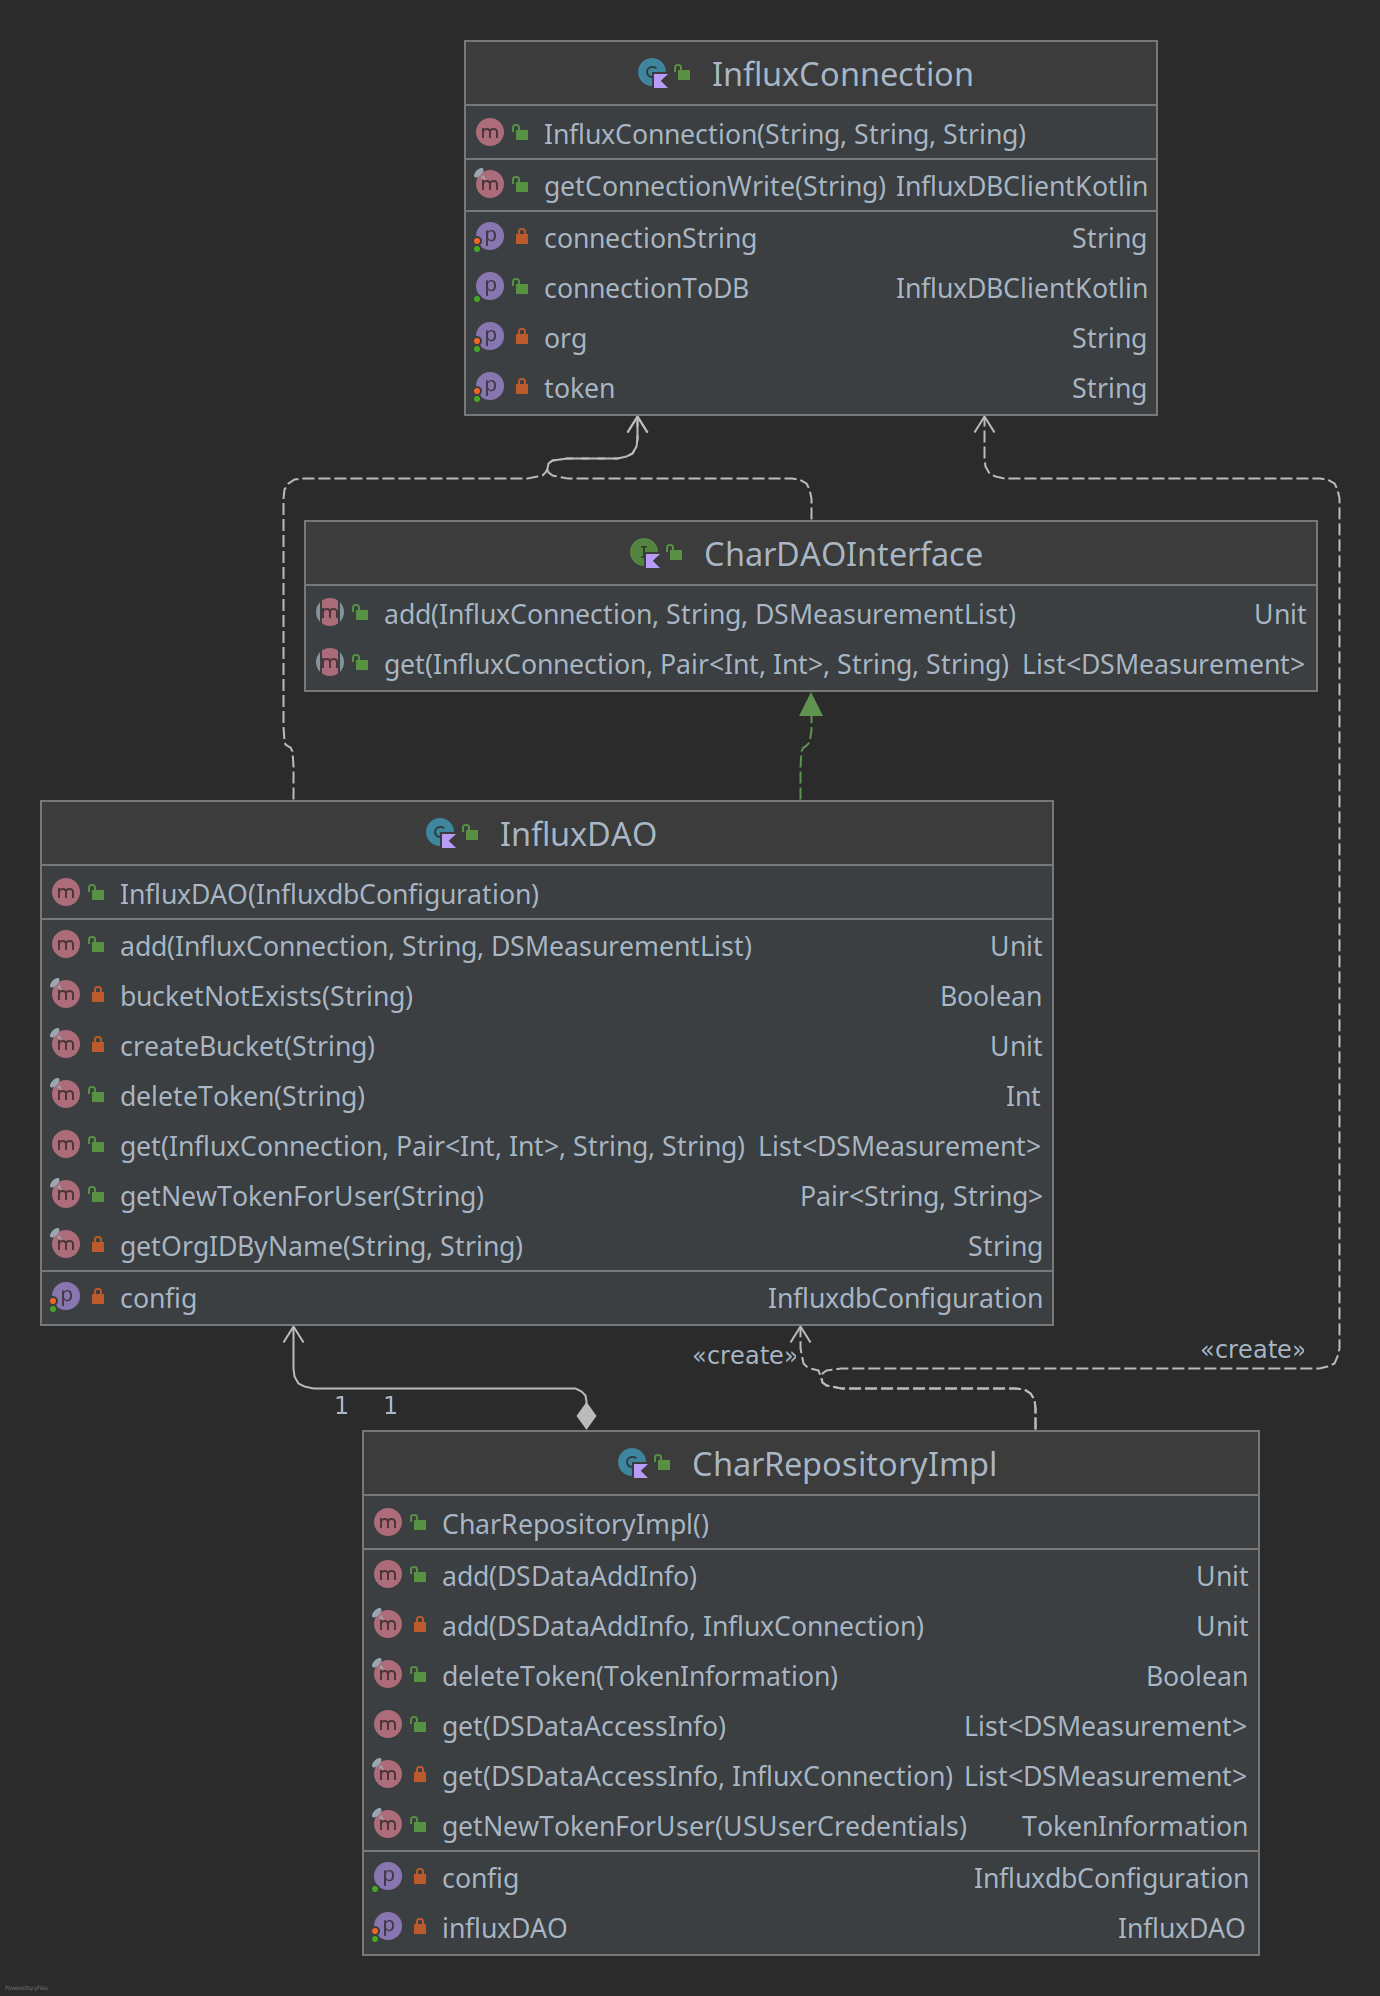
\includegraphics[width=\textwidth]{img/dataLayerDiagram.png}
\captionsetup{justification=centering}
	\caption{Диаграмма классов слоя доступа к данным приложения. }
	\label{fig:dataLayer}
\end{center}
\end{figure}

\begin{figure}[H]
	\centering
	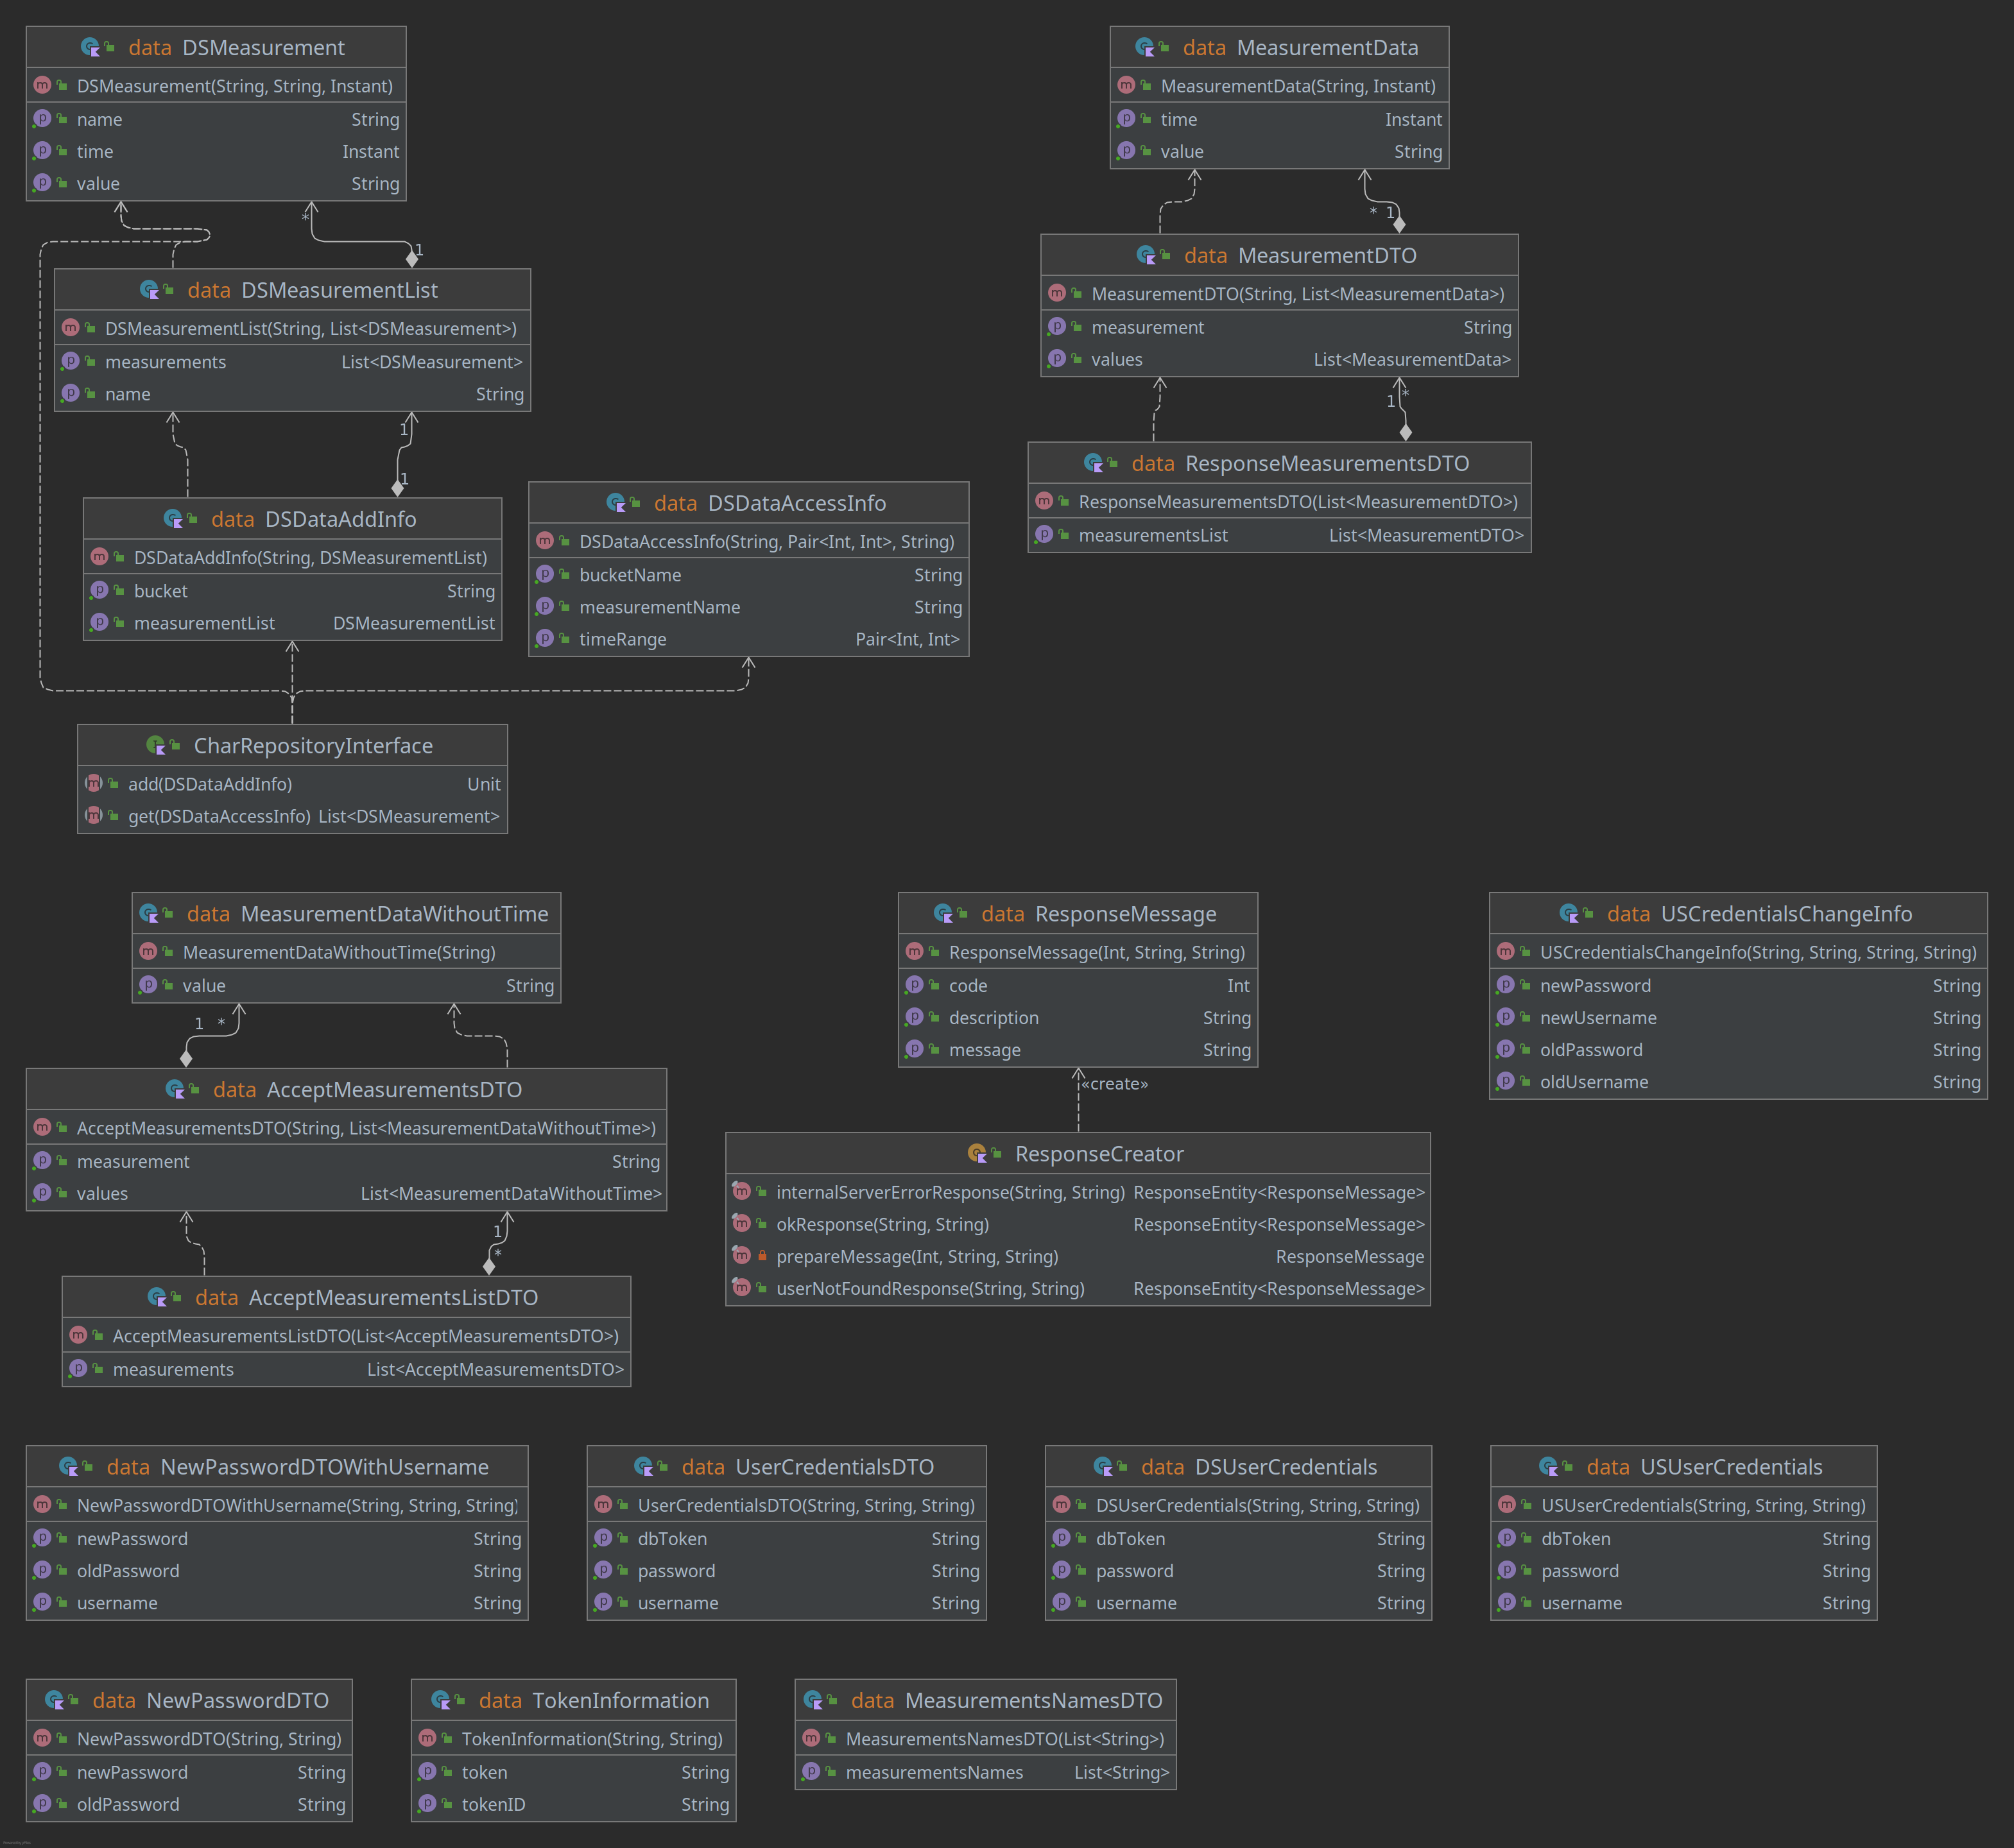
\includegraphics[width=\textwidth]{img/domainLayerDiagram.png}
	\caption{Диаграмма классов бизнес-логики приложения. }
	\label{fig:domainLayer}
\end{figure}

\begin{figure}[H]
	\centering
	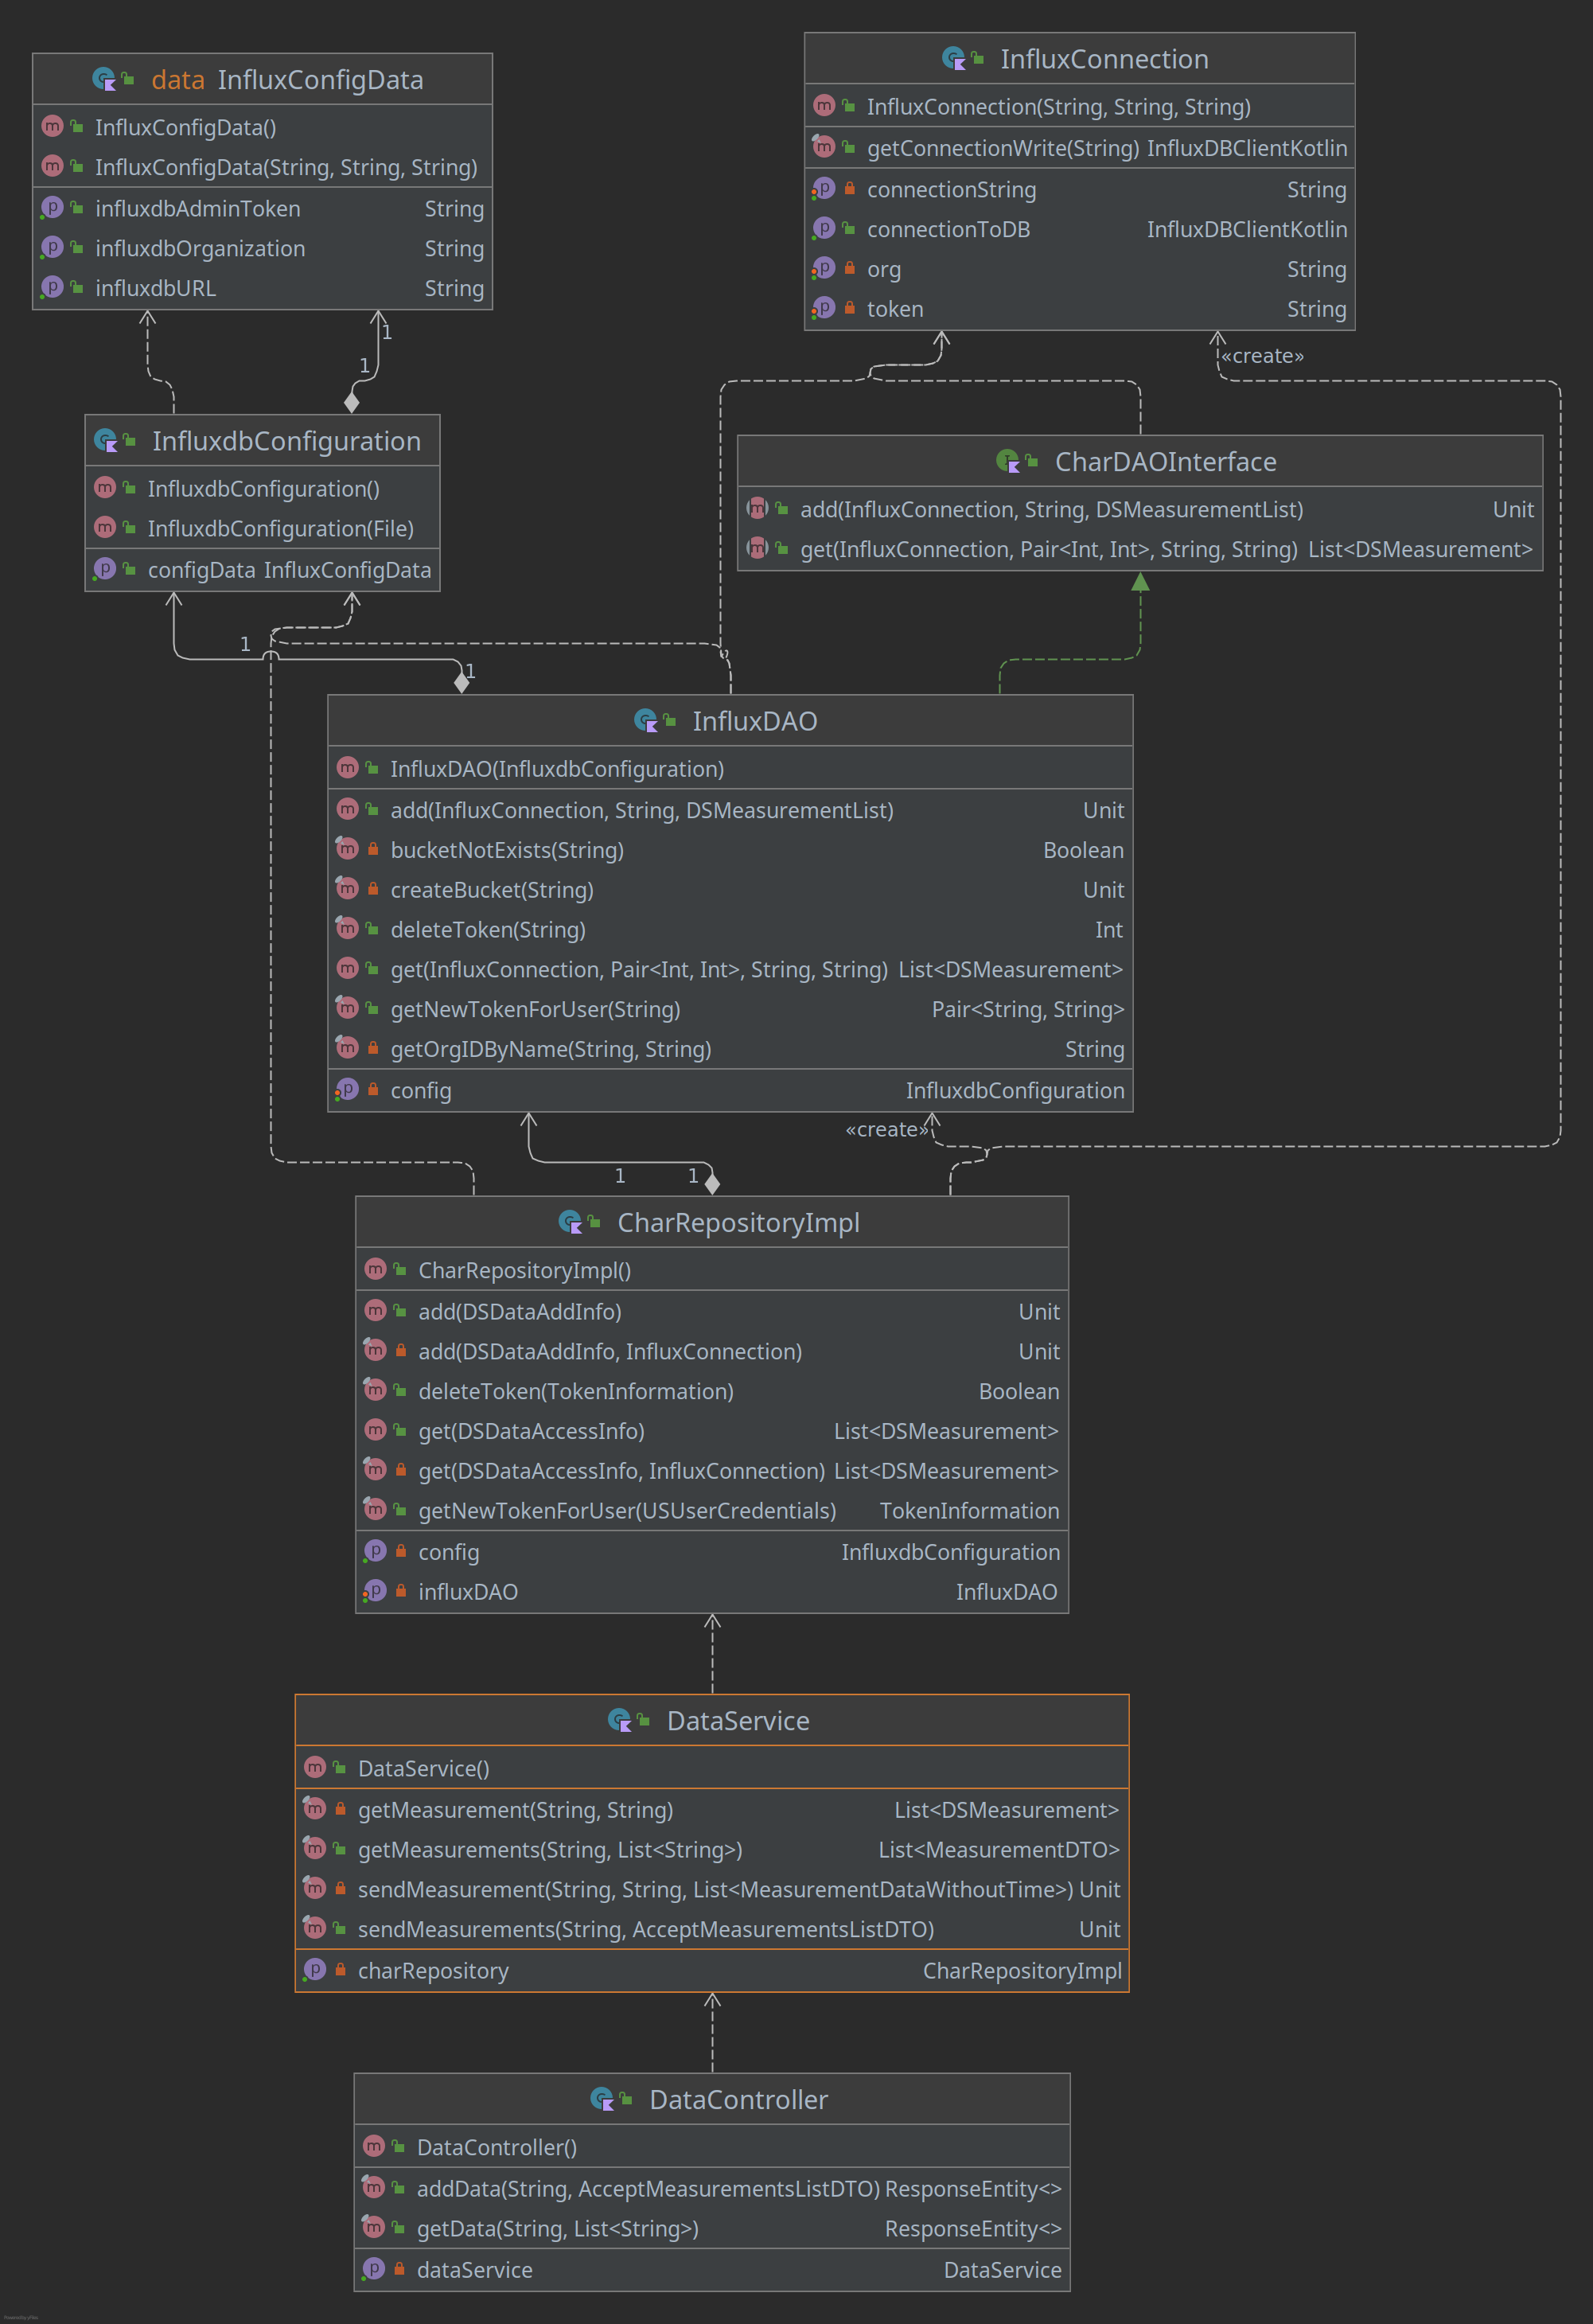
\includegraphics[width=\textwidth]{img/dataAndControllerLinkageDiagram.png}
	\caption{Диаграмма классов, показывающая связь контроллера и слоя доступа к данным. }
	\label{fig:dataAndController}
\end{figure}

\begin{figure}[H]
	\centering
	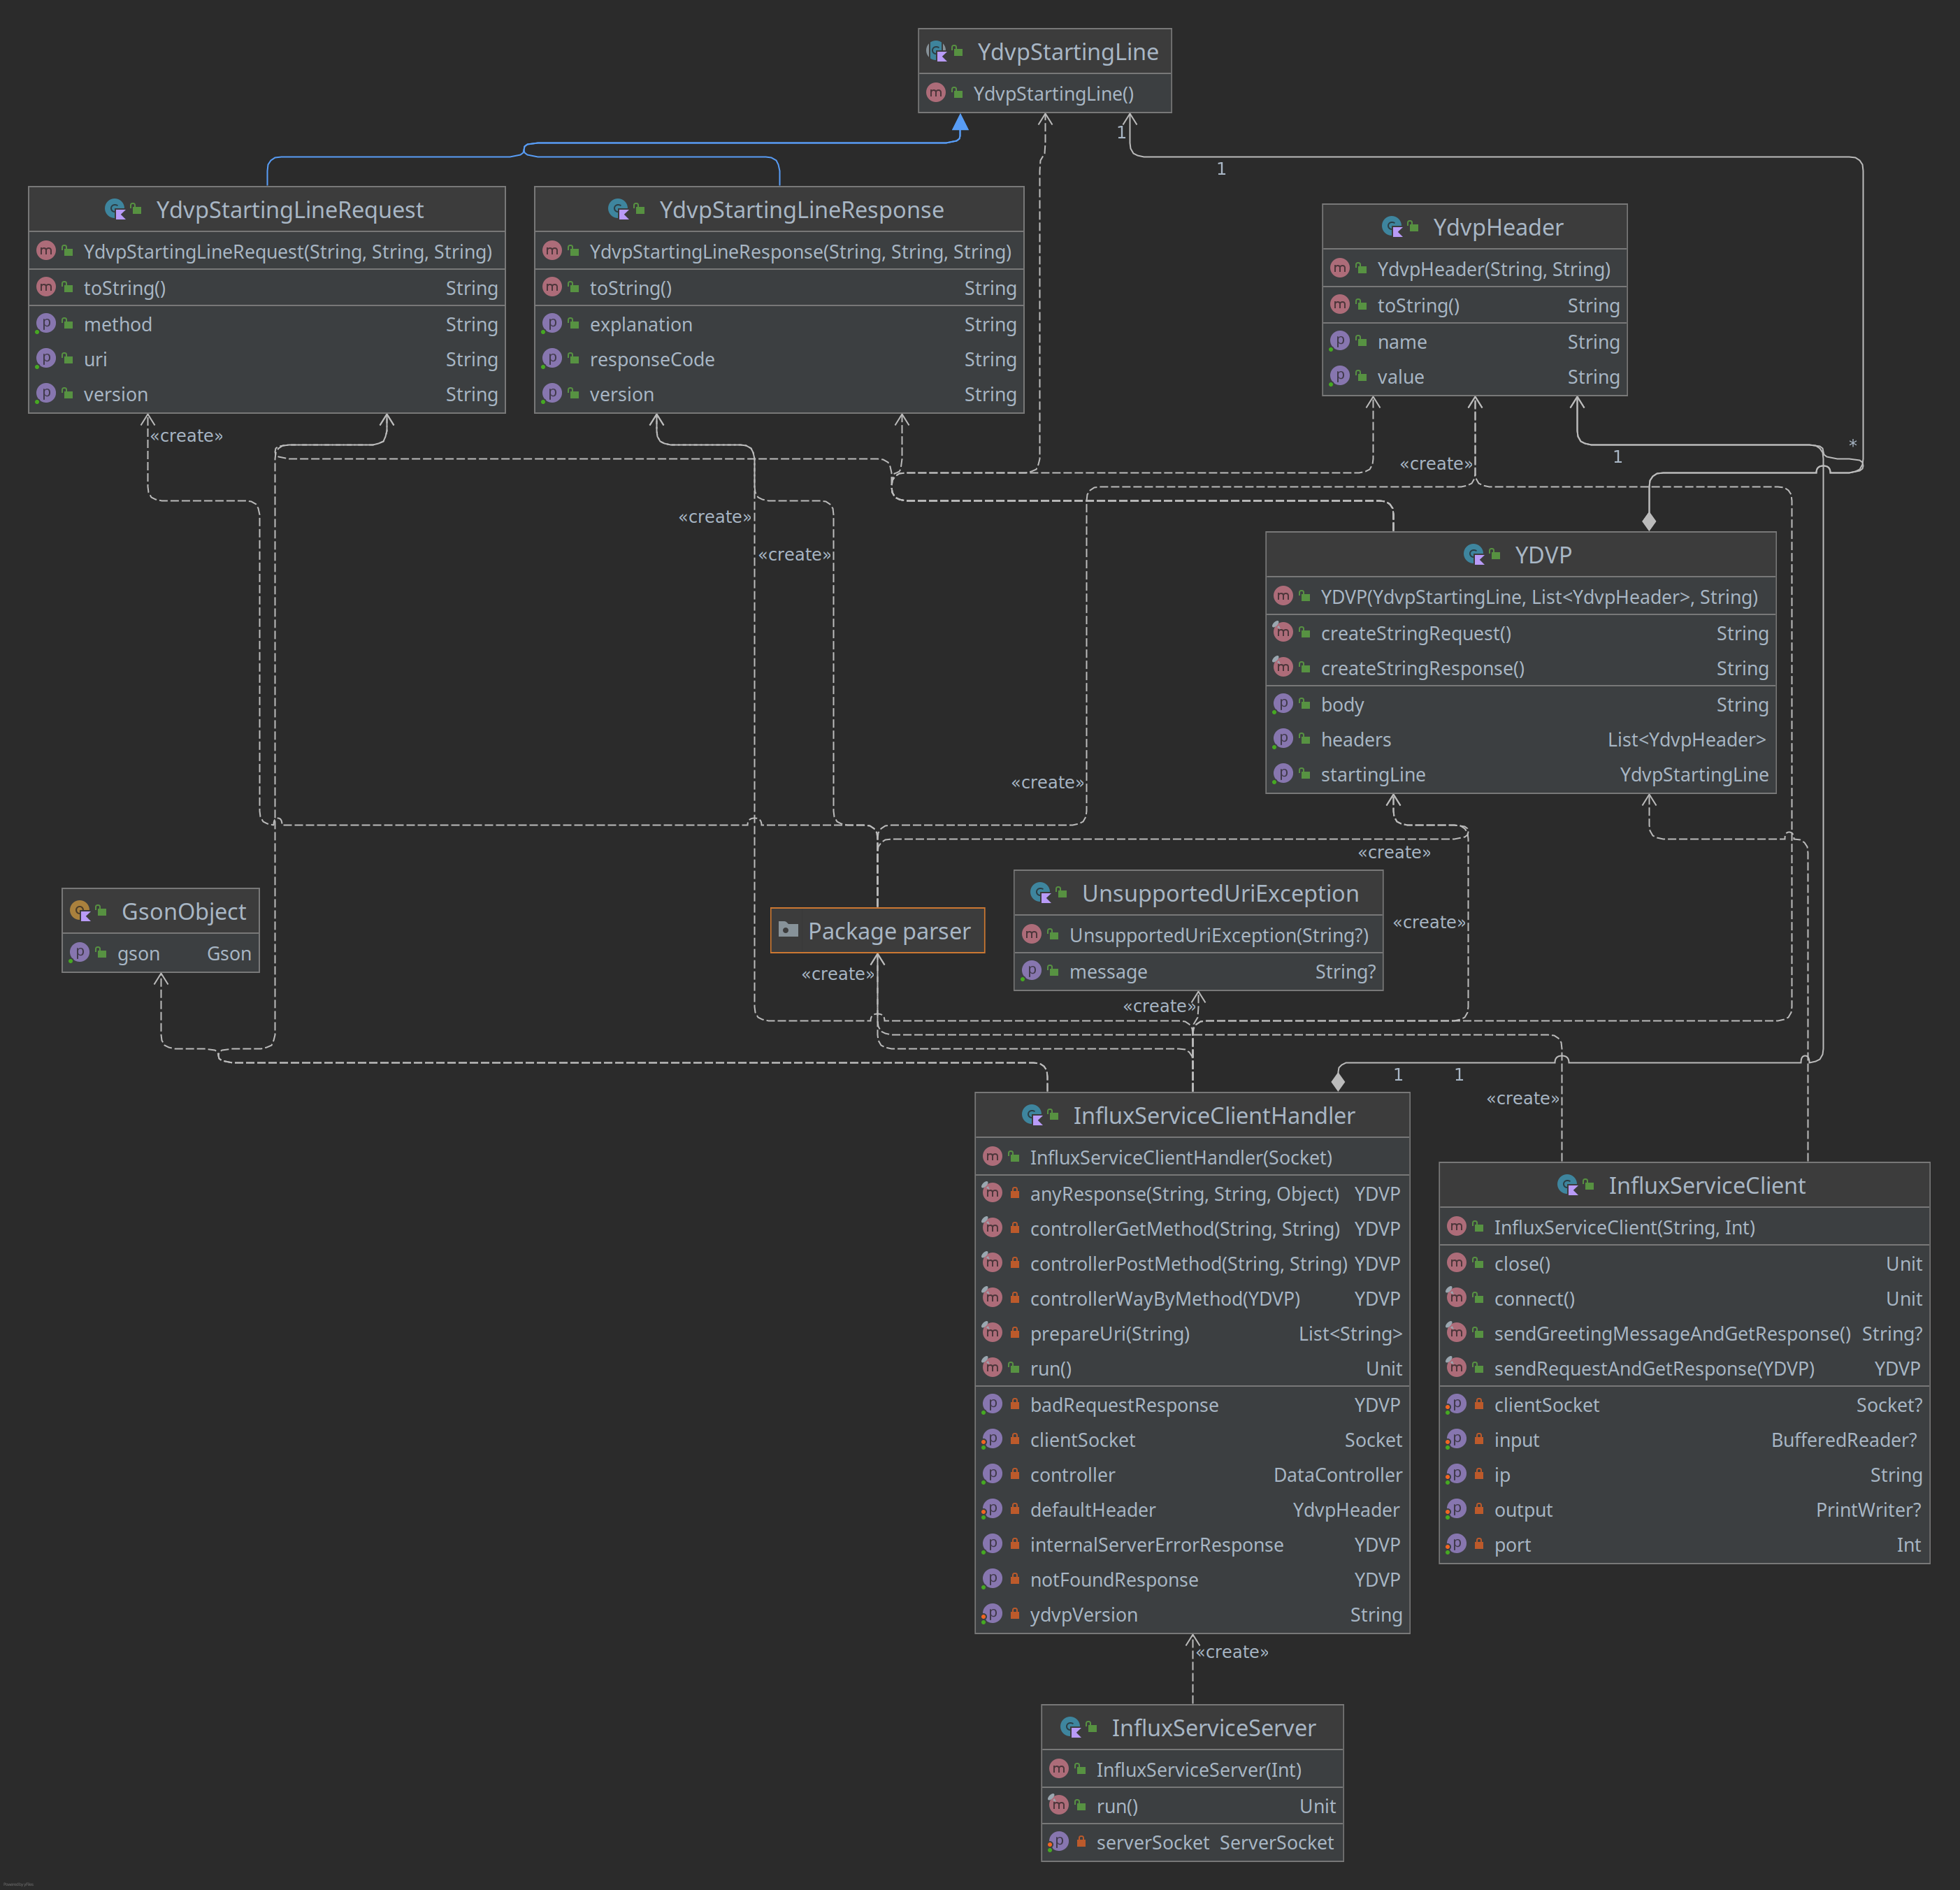
\includegraphics[width=\textwidth]{img/serverDiagram.png}
	\caption{Диаграмма классов серверной части приложения. }
	\label{fig:serverAndProtocol}
\end{figure}

\subsection{Особенности реализации}
В листинге \ref{code:InfluxServiceServer} предоставлено описание класса сервера приложения.

Данный класс инициализирует классы для инъекции зависимостей в модули, используемые сервисами и контроллерами, а также передаёт приходящих клиентов обработчику (классу InfluxServiceClientHandler) в отдельном потоке, таким образом достигается возможность одновременной обработки запросов от нескольких клиентов.

\begin{code}
	\captionof{listing}{Реализация класса InfluxServiceServer}
	\label{code:InfluxServiceServer}
	\inputminted
	[
	frame=single,
	framerule=0.5pt,
	framesep=20pt,
	fontsize=\small,
	tabsize=4,
	linenos,
	numbersep=5pt,
	xleftmargin=10pt,
	firstline=185,
	lastline=221,
	breaklines=true
	]
	{text}
	{code/server.kt}
\end{code}

В листинге \ref{code:InfluxServiceClientHandler} предоставлено описание класса обработчика запроса клиента.

Данный класс включает в себя необходимый для навигации по ресурсам контроллер, а также типовые объекты YDVP-ответов и методы обработки запроса клиента.

\begin{code}
	\captionof{listing}{Реализация класса InfluxServiceClientHadler}
	\label{code:InfluxServiceClientHandler}
	\inputminted
	[
	frame=single,
	framerule=0.5pt,
	framesep=20pt,
	fontsize=\small,
	tabsize=4,
	linenos,
	numbersep=5pt,
	xleftmargin=10pt,
	firstline=26,
	lastline=183,
	breaklines=true
	]
	{text}
	{code/server.kt}
\end{code}

\subsection{Пример использования приложения}
В листингах \ref{code:server}--\ref{code:client} предоставлен пример реализации взаимодействия пользователя с сервером.
\begin{code}
	\captionof{listing}{Пример организации серверной части.}
	\label{code:server}
	\inputminted
	[
	frame=single,
	framerule=0.5pt,
	framesep=20pt,
	fontsize=\small,
	tabsize=4,
	linenos,
	numbersep=5pt,
	xleftmargin=10pt,
	breaklines=true
	]
	{text}
	{code/helloServer.kt}
\end{code}

\begin{code}
	\captionof{listing}{Пример вызовов со стороны клиента.}
	\label{code:client}
	\inputminted
	[
	frame=single,
	framerule=0.5pt,
	framesep=20pt,
	fontsize=\small,
	tabsize=4,
	linenos,
	numbersep=5pt,
	xleftmargin=10pt,
	breaklines=true
	]
	{text}
	{code/helloClient.kt}
\end{code}

На рисунках \ref{fig:serverOutput}--\ref{fig:clientOutput} предоставлен результат выполнения клиентской и серверной частей предоставленного примера.

\begin{figure}[H]
\begin{center}
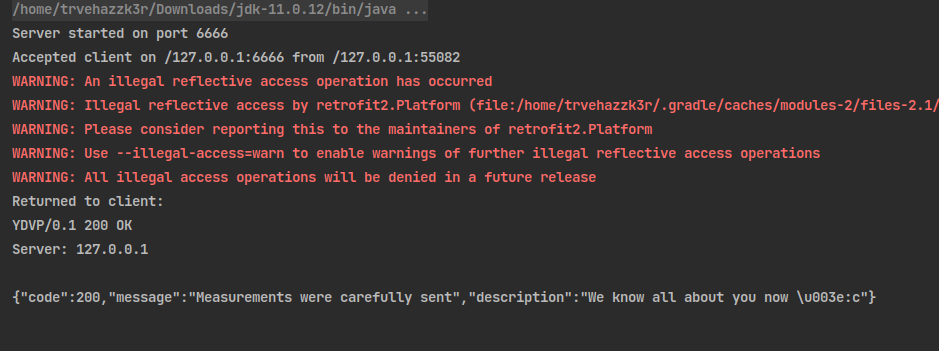
\includegraphics[width=\textwidth]{img/serverOutput.png}
\captionsetup{justification=centering}
	\caption{Результат выполнения запроса на стороне сервера. }
	\label{fig:serverOutput}
\end{center}
\end{figure}

\begin{figure}[H]
\begin{center}
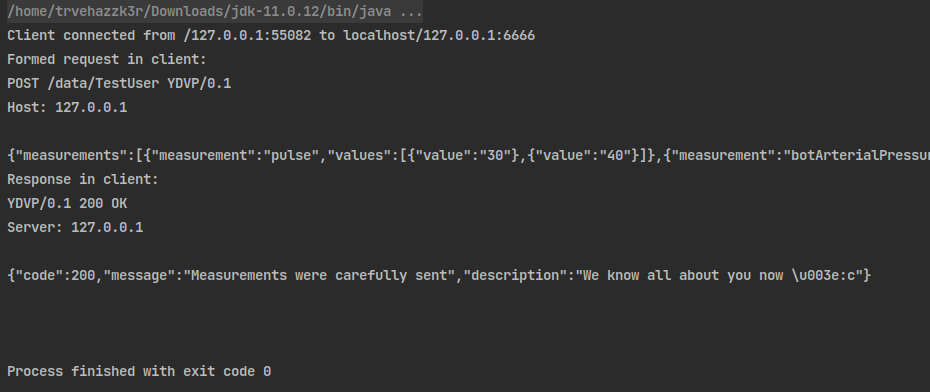
\includegraphics[width=\textwidth]{img/clientOutput.png}
\captionsetup{justification=centering}
	\caption{Результат выполнения запроса на клиентской стороне. }
	\label{fig:clientOutput}
\end{center}
\end{figure}

\subsection*{Вывод}
В качестве средств реализации были выбраны язык программирования Kotlin и среда разработки Intellij IDEA.

В разделе были предоставлены краткие сведения о модулях программы, в которых была предоставлена информация об используемых шаблонах проектирования, а также системе взаимодействии классов в приложении.

Была рассмотрена структура и состав классов, представленных в форме UML-диаграмм, и приведены особенности реализации, указывающие на возможность одновременной работы реализованного сервера с несколькими клиентами.

Пример, предоставленный в разделе, показал возможные пути использования реализованных компонентов.